\documentclass[12pt, a4paper, twoside]{article}
\usepackage{../labreport}
\usepackage{pdfpages}

\setlabreportopts[authors={Nandor Kovacs \& Céline Schuster},
    title={Glühlämpchen},
    subtitle={Aufbau von einfachen Schaltkreisen, und die Messung von Strom und Spannung},
    date={\today},
    labdate={24. März 2022}
]

\begin{document}
  \maketitlepage
  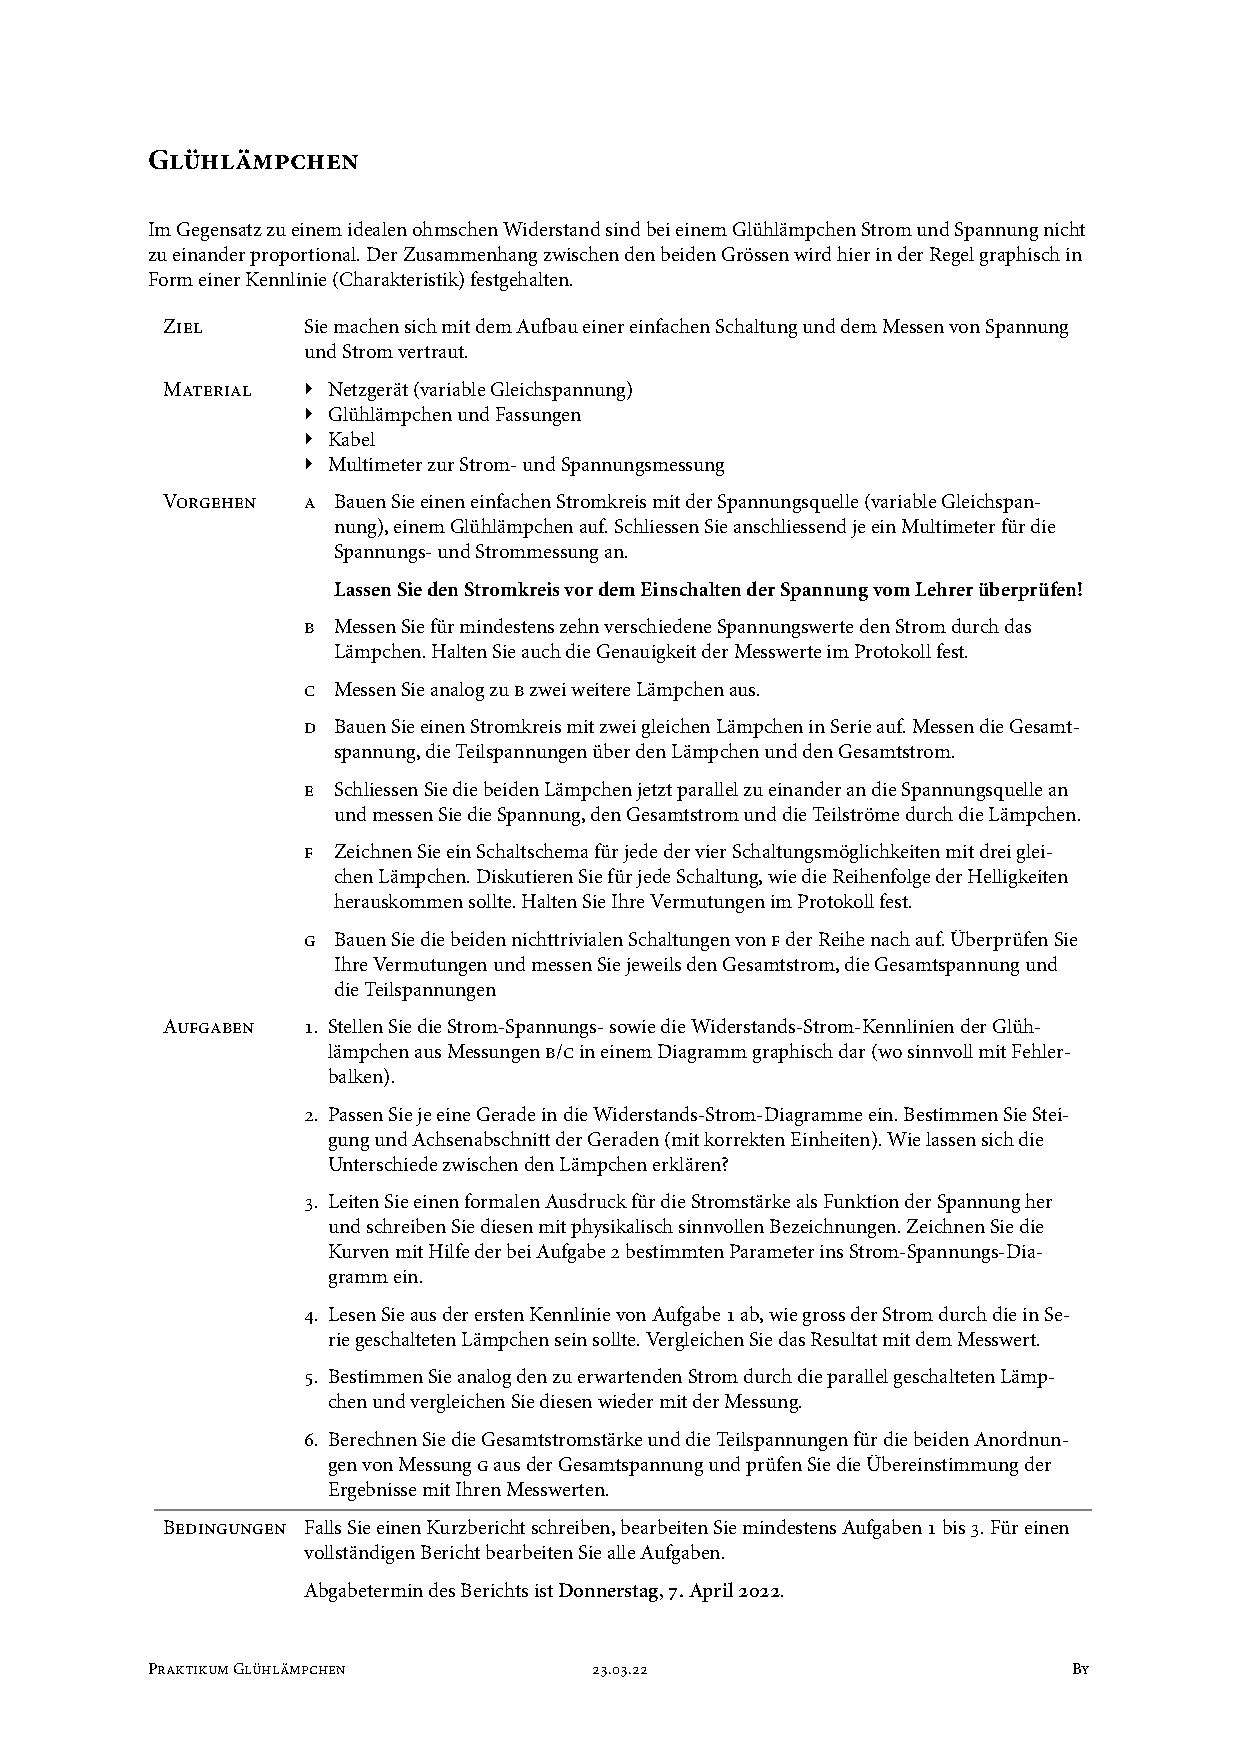
\includepdf[pages={1}]{aufgabenstellung.pdf}
  \section{Einleitung}
  \section{Theorie}
  \section{Experiment}
  \section{Messungen}
  \section{Aufgaben}
  \section{Fazit}
  \section{Reflektion}
  \section{Anhang}
  Versuchsanleitung und Originalprotokoll vom \labdate
\end{document}